
\documentclass{beamer}

\usetheme{AnnArbor}
\usecolortheme{beaver}

\title{Freedom of Information Act Wiki}
\subtitle{foiawiki.org.uk}
\author[Presenter: Iain R. Learmonth]{{\bf Iain R. Learmonth} \\ Johnny McKenzie \\ Tom Jones}
\date[22nd June 2014]{22nd June 2014 \\ Code the City Aberdeen 2014}

\begin{document}

\begin{frame}
\maketitle
\end{frame}

\begin{frame}
	\frametitle{What did exist?}
Aberdeen City Council publish a FOI disclosure log but it is not searchable and rather difficult to navigate.
\end{frame}

\begin{frame}
	\frametitle{Improvements needed}
	\begin{itemize}
		\item{Make searchable}
		\item{Allow crowdsourced tagging}
		\item{Aggregate disclosures from multiple sources}
		\item{Allow re-use of the data}
	\end{itemize}
\end{frame}

\begin{frame}
	\frametitle{Identifying data}
	\begin{center}
		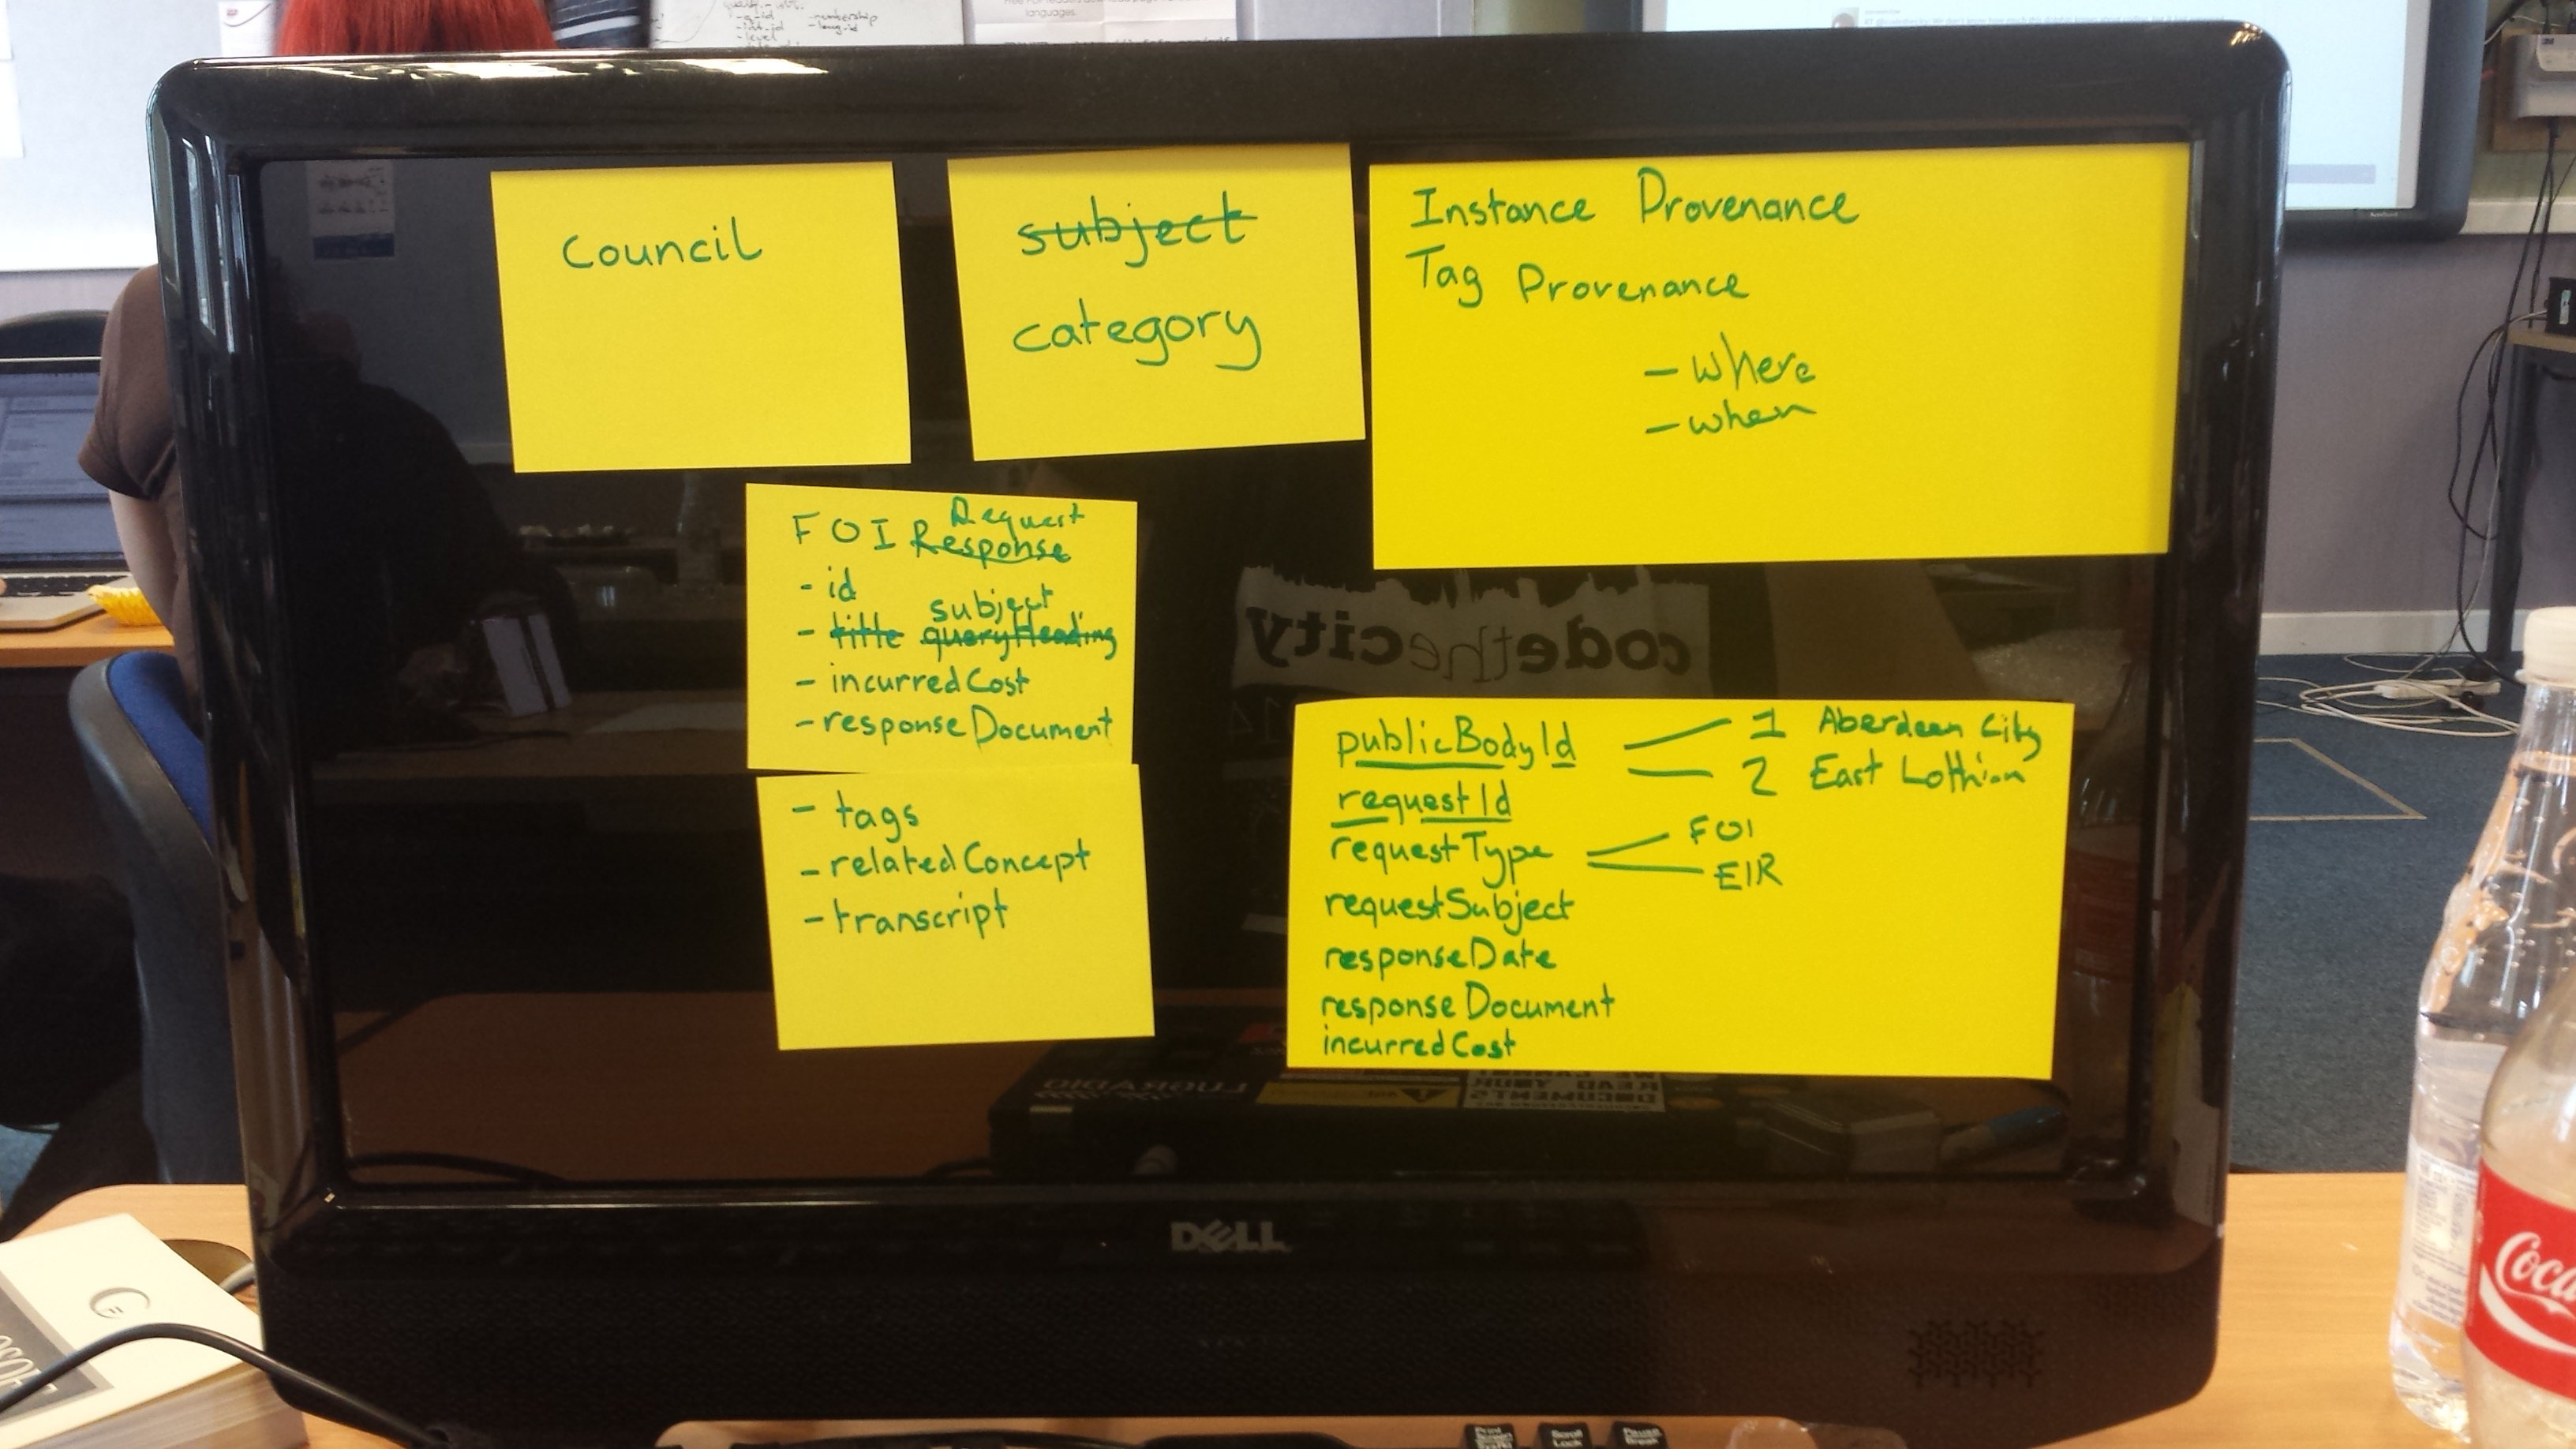
\includegraphics[width=0.7\textwidth]{information.jpg}
	\end{center}
\end{frame}

\begin{frame}
	\frametitle{Building schemas}
	\begin{itemize}
		\item{Web Ontology Language (OWL)}
		\item{MySQL}
	\end{itemize}
\end{frame}

\begin{frame}
	\frametitle{Documenting the schema}
	Using LODE\footnote{http://www.essepuntato.it/lode}:
	\begin{center}
		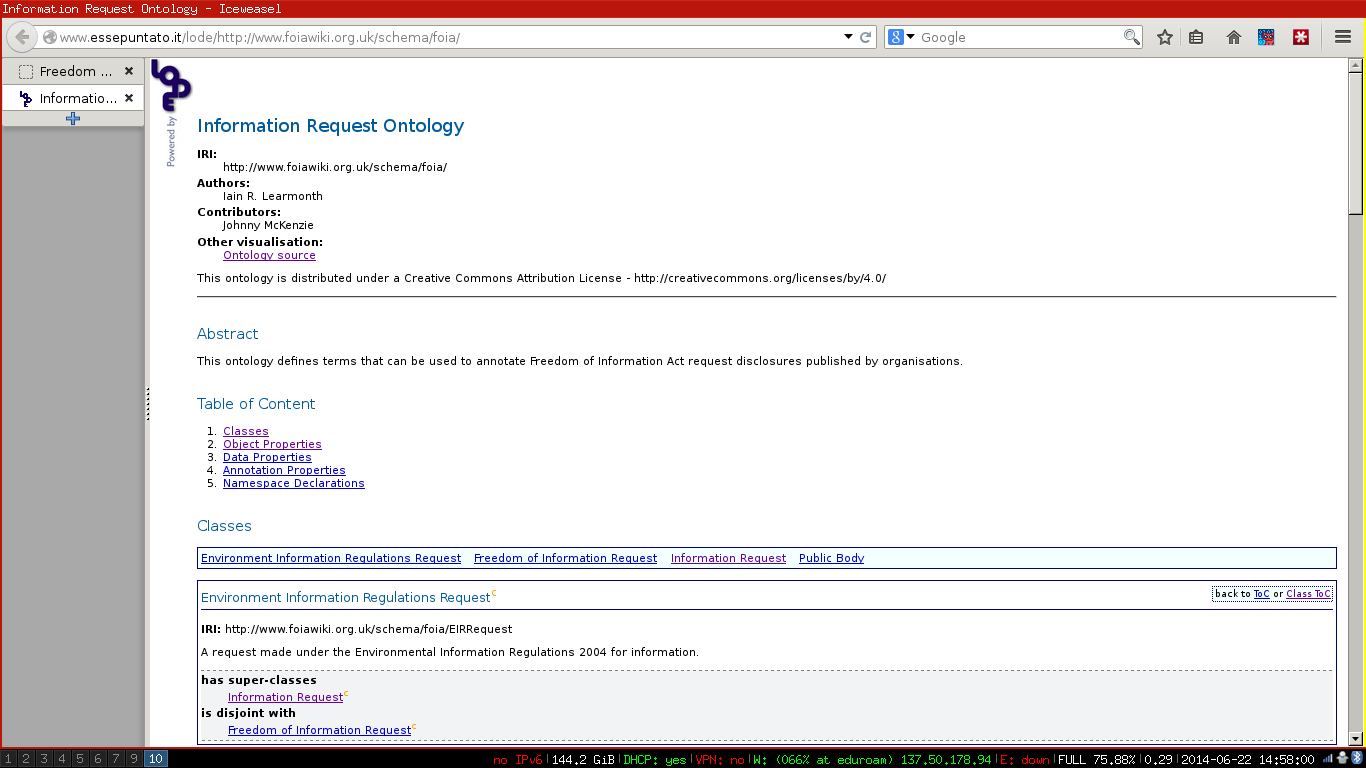
\includegraphics[width=0.7\textwidth]{ontology.png}
	\end{center}
\end{frame}

\begin{frame}
	\frametitle{Publishing linked data}
	Using D2R Server\footnote{http://d2rq.org/d2r-server}:

\ 
	
	{\tt \tiny
map:InformationRequests a d2rq:ClassMap; \\
\        d2rq:dataStorage map:database; \\
\        d2rq:uriPattern "request/@@request.publicBodyId@@/@@request.requestId|urlify@@"; \\
\        d2rq:class foia:InformationRequest; \\
\ .}
\end{frame}

\begin{frame}
	\frametitle{An Example Frontend}
	\begin{center}
		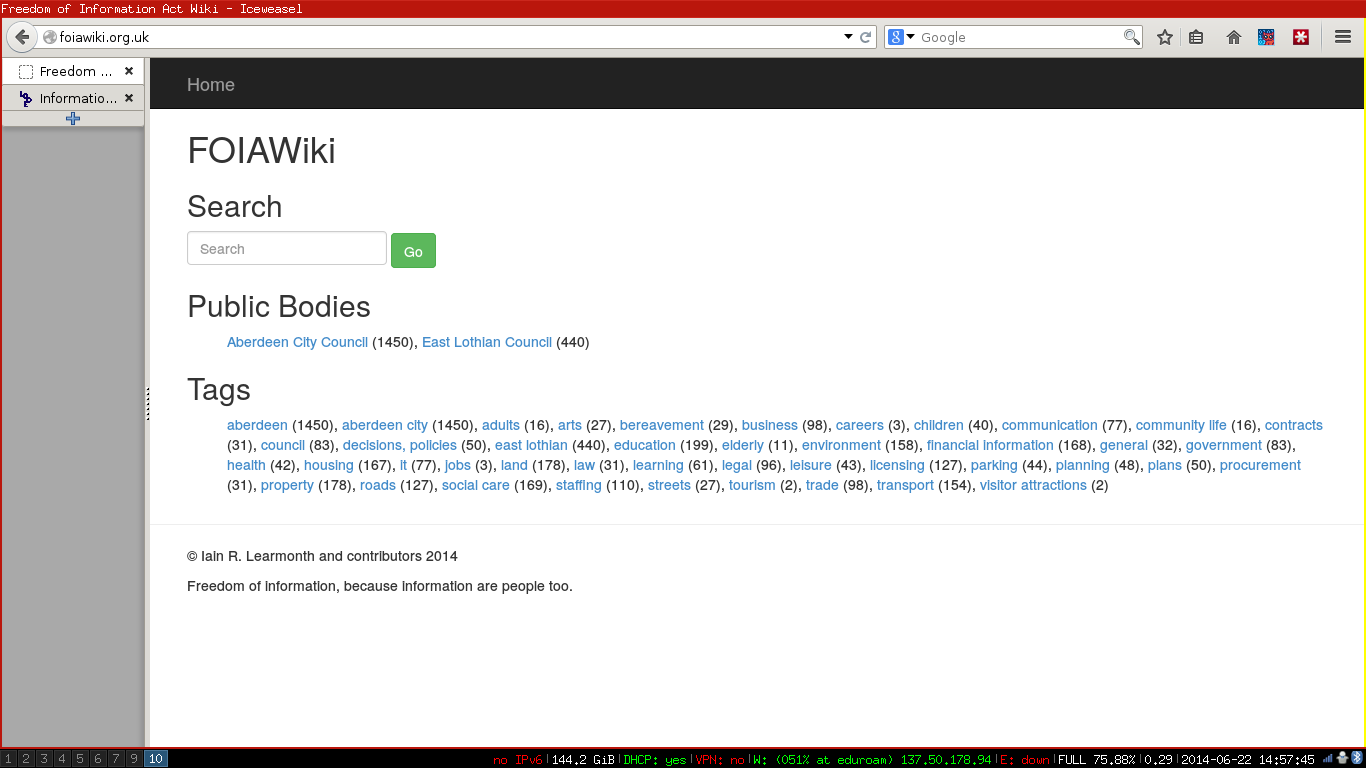
\includegraphics[width=0.8\textwidth]{interface.png}
	\end{center}
\end{frame}

\begin{frame}
	\begin{center}
		irl@fsfe.org
	\end{center}
\end{frame}

\end{document}

